\subsection{Comparison of Resulting Concept Lattices}
\label{sec:lattice_comparison}


The two lattices are constructed over the same object set of 11\,000 documents. 
The \ac{mlb}-constrained lattice in Figure~\ref{fig:mlb_concept_lattice} contains all concepts, the topic model-based lattice in Figure~\ref{fig:iceberg_concept_lattice} is computed as an iceberg lattice, retaining only concepts whose intents satisfy a minimum support threshold. 
This restriction is necessary because the complete topic model-based lattice contains more than 550 concepts (Figure~\ref{fig:concepts_support}), which would hinder visualization and interpretation.

\begin{figure}[t]
    \centering
    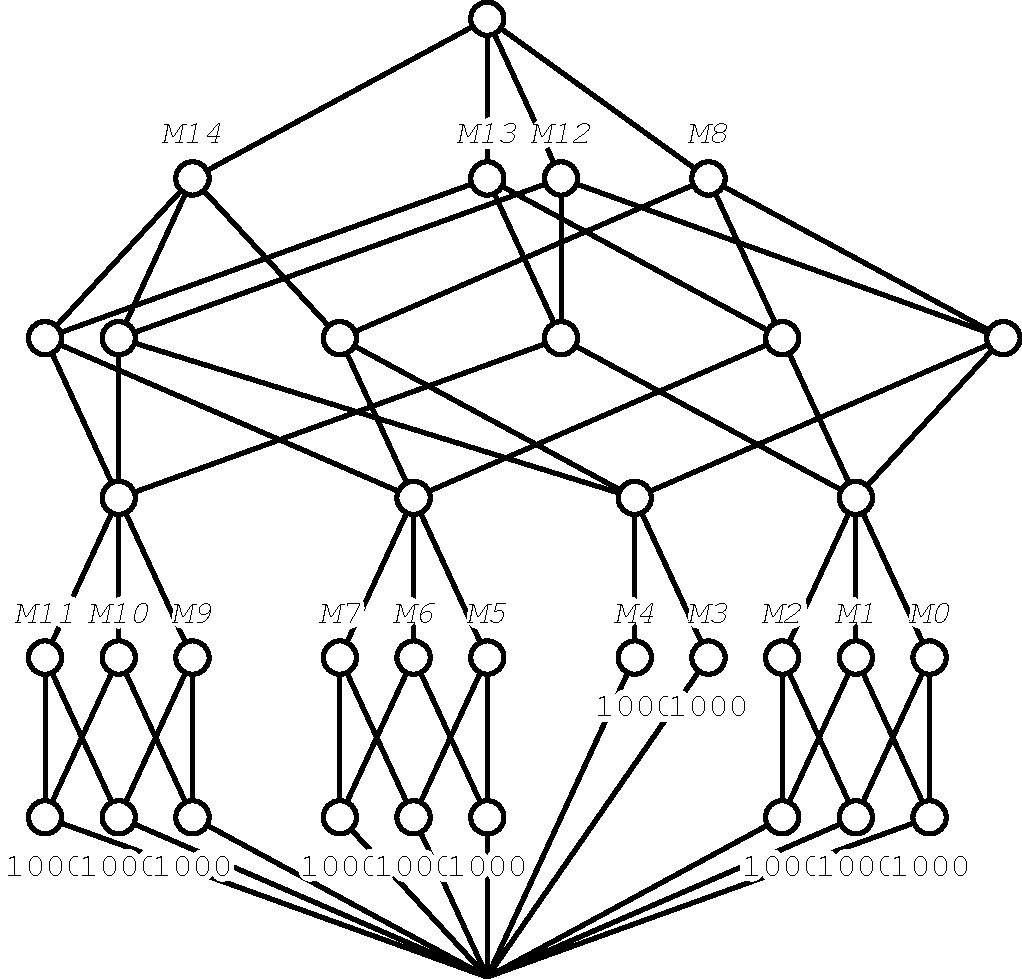
\includegraphics[width=0.6\textwidth]{resources/banksearch/ground_truth/mlb_expanded.pdf}
    \caption{\ac{mlb}-constrained concept lattice. Top labels denote attributes; bottom labels indicate the number of documents in the corresponding concept extent. Evaluation against manually annotated ground-truth labels indicates that numbered nodes correspond to document clusters sharing the same topic.} % kind of obvious, because that is the smallest attribute set they share
    \label{fig:mlb_concept_lattice}
\end{figure}

In the \ac{mlb}-constrained concept lattice (Figure~\ref{fig:mlb_concept_lattice}), attributes are labeled $M_i$ as generated by the script constructing the formal context from the \ac{mlb} constraints. 
The lattice contains 15 attributes, of which only $M3$ and $M4$ correspond directly to ground-truth topics (\texttt{Biology} and \texttt{Astronomy}). 
This correspondence was identified by matching concept extents to the original topic assignments.
Most remaining topics emerge as intersections of attributes; for example, \texttt{Sport} corresponds to $M0 \cap M1$, while \texttt{Soccer} and \texttt{Motor Racing} correspond to $M1 \cap M2$ and $M0 \cap M2$, respectively.
Consequently, most original topics appear near the bottom of the lattice.

\begin{figure}[t]
    \centering
    \includesvg[width=\textwidth]{resources/banksearch/topic_model/banksearch_0.05_iceberg.svg}
    \caption{Iceberg concept lattice derived from the topic model. Top labels denote cluster IDs in the concept intent; bottom labels indicate the number of documents in the concept extent.}
    \label{fig:iceberg_concept_lattice}
\end{figure}

The topic model-based lattice (Figure~\ref{fig:iceberg_concept_lattice}) contains 24 concepts with support of at least $\delta_{ms}=0.05$. 
Unlike the \ac{mlb}-constrained lattice, the original dataset topics are not explicitly represented as individual concepts.
The iceberg lattice contains only two non-trivial levels besides the top and bottom concepts, resulting in substantially less hierarchical depth than the \ac{mlb}-constrained lattice due to iceberg pruning. 
This reduction in structure is expected due to the pruning effect of the iceberg constraint.

\begin{figure}[hbt]
    \centering
    \includesvg[width=0.64\textwidth]{results/context_comparison/CONCEPT_SIM/heatmap_0.05.svg}
    \caption{Pairwise Jaccard similarities between concept extents of the \ac{mlb}-constrained lattice and the topic model-based iceberg lattice. Apart from the trivial similarity of the top concepts, most pairs exhibit near-zero similarity. \textcolor{red}{TODO: update path dep. on min-supp}}
    \label{fig:concept_lattice_similarity}
\end{figure}

% Glckstad2013UnsupervisedKS use Jaccard for overlapping intents
To compare both lattices, we compute the Jaccard similarity~\cite{Glckstad2013UnsupervisedKS} between all pairs of concept extents.
For extents $A$ and $B$, the similarity is defined as $J(A,B) = \frac{|A \cap B|}{|A \cup B|}$.
Figure~\ref{fig:concept_lattice_similarity} shows that most similarities are close to zero, indicating minimal overlap between document clusters.
Excluding the trivial similarity of the top concepts, only \textcolor{red}{three} concept pairs reach a similarity above $0.6$ (Table~\ref{tab:concept_jaccard_similarity}). 
These pairs correspond to concepts located in the middle region of the \ac{mlb}-constrained lattice. 
For example, the concept generated by $A'{M4, M8, M12, M14}$ (at the $m4$ node \texttt{Astronomy}), aligns most closely with topic-model concept $c10$, which captures computer science-related topic words.
Overall, the two lattices exhibit very limited structural similarity.

%% min-sup = 0.1
\begin{table}[b]
\centering
% Jaccard is defined on extent, therefore we compare J(A,B) but refer to the intents as concept identifiers
\caption{Concept pairs with Jaccard similarity above $0.6$, where $A'$ denotes the \ac{mlb}-constrained concept intent and $B'$ the topic model-based concept intent. \textcolor{red}{update with min-supp=0.05, ggf. new computation cf. Fig. 7?}}
\label{tab:concept_jaccard_similarity}
\begin{tabular}{lll}
\toprule
$A'$ & $B'$ & $J(A,B)$ \\
\midrule
$\{M12, M13, M14\}$ & $\{c7\}$ & 0.77 \\
$\{M1, M8, M12, M13\}$  & $\{c9\}$ & 0.65 \\
$\{M4, M8, M12, M14\}$  & $\{c10\}$ & 0.64 \\
\bottomrule
\end{tabular}
\end{table}



\subsection{Consistency-Lattice vs. Coherence-Lattice}
\label{sec:consistency_vs_coherence}

The consistency lattice in Figure~\ref{fig:consistency_coherence_lattices} (left) is computed by intersecting the \ac{mlb}-constrained lattice with the lattice derived from the topic model, following the procedure described in Section~\ref{sec:integrated_lattice_computation}.
Formally, $\mathcal{C}_{\cap} = \mathcal{C}_{\Sigma} \cap \mathcal{C}_{TM}$. In our case, this intersection is near-trivial, containing only the top and bottom concepts.
To investigate partial overlaps, we define the \textit{coherence-lattice} $\mathfrak{B}(\mathbb{K}_{coh})$. We construct a new formal context $\mathbb{K}_{coh} = (G, M_{coh}, I_{coh})$, where the attributes $M_{coh}$ are derived from pairs of concepts $(A, B)$ with $A \in \mathcal{C}_{\Sigma}$ and $B \in \mathcal{C}_{TM}$ that satisfy a Jaccard threshold $\theta$:
\begin{equation}
    M_{coh} = \{ A \cap B \mid A \in \mathcal{C}_{\Sigma}, B \in \mathcal{C}_{TM}, J(A, B) > \theta \}
\end{equation}
We set $\theta = 0.6$ which allows us to visualize document clusters that are \textit{nearly} consistent across both knowledge sources.
Since the top node of the coherence lattice contains $11\,000$ documents the resulting lattice covers the complete corpus.

\begin{figure}[t]
\centering

\begin{subfigure}{0.45\textwidth}
    \centering
    \includesvg[width=0.35\textwidth]{results/context_comparison/intersection.svg}
    % \caption{\textit{Consistency}-lattice.}
\end{subfigure}
\hfill
\begin{subfigure}{0.45\textwidth}
    \centering
    \includesvg[width=0.7\textwidth]{results/context_comparison/CONCEPT_SIM/coherence.svg}
    % \caption{\textit{Coherence}-lattice.}
\end{subfigure}

\caption{The \emph{consistency} lattice (left) and \emph{coherence} lattice (right) from the \ac{mlb}-constrained lattice and the topic model-based lattice for the BankSearch dataset.}
\label{fig:consistency_coherence_lattices}

\end{figure}
